\documentclass{article}
\usepackage{hyperref}
\usepackage{graphicx}
\usepackage{amsmath}
\usepackage{amssymb}
\usepackage{listings}
\usepackage{xcolor}          % Using xcolor for more robust color specification

%%%%%%%%%%%%%%%%%%%%%%%%%%%%%%%%%%%%%%%%%%%%%%%%%%%%%%%%%%%%%%%%%%%%%%%%%%%%%%%%
%% Custom Commands

% Custom colors
\definecolor{deepblue}{rgb}{0,0,0.5}
\definecolor{deepred}{rgb}{0.6,0,0}
\definecolor{deepgreen}{rgb}{0,0.5,0}
\definecolor{forestgreen}{RGB}{34,139,34}
\definecolor{orangered}{RGB}{239,134,64}
\definecolor{darkblue}{rgb}{0.0,0.0,0.6}
\definecolor{gray}{rgb}{0.4,0.4,0.4}

% Named Colors for the comments below (Attempted to match git symbol colors)
\definecolor{RScolor}{HTML}{8EB361}  % Sonat (adjusted for clarity)
\definecolor{DPMcolor}{HTML}{E28B8D} % Dan
\definecolor{JCcolor}{HTML}{82A8D9}  % Josh (adjusted for clarity)
\definecolor{AAcolor}{HTML}{8D7F44}  % Andrea
\definecolor{CRcolor}{HTML}{AC39CE}  % Cristian
\definecolor{RKcolor}{HTML}{3ECC8D}  % Bob (adjusted for clarity)
\definecolor{DMcolor}{HTML}{276605}  % Diego (adjusted for clarity)
\definecolor{PTcolor}{HTML}{990000}  % Paul

\def\DRAFT{} % Uncomment this if you want to see the notes people have been adding
% Comment command for developers (Should only be used under active development)
\ifdefined\DRAFT
  \newcommand{\nameLabeler}[3]{\textcolor{#2}{[[#1: #3]]}}
\else
  \newcommand{\nameLabeler}[3]{}
\fi

\newcommand{\alfoa}[1] {\nameLabeler{Andrea}{AAcolor}{#1}}
\newcommand{\cristr}[1] {\nameLabeler{Cristian}{CRcolor}{#1}}
\newcommand{\mandd}[1] {\nameLabeler{Diego}{DMcolor}{#1}}
\newcommand{\maljdan}[1] {\nameLabeler{Dan}{DPMcolor}{#1}}
\newcommand{\cogljj}[1] {\nameLabeler{Josh}{JCcolor}{#1}}
\newcommand{\bobk}[1] {\nameLabeler{Bob}{RKcolor}{#1}}
\newcommand{\senrs}[1] {\nameLabeler{Sonat}{RScolor}{#1}}
\newcommand{\talbpaul}[1] {\nameLabeler{Paul}{PTcolor}{#1}}
% Commands for making the LaTeX a bit more uniform and cleaner
\newcommand{\TODO}[1]    {\textcolor{red}{\textit{(#1)}}}
\newcommand{\xmlAttrRequired}[1] {\textcolor{red}{\textbf{\texttt{#1}}}}
\newcommand{\xmlAttr}[1] {\textcolor{cyan}{\textbf{\texttt{#1}}}}
\newcommand{\xmlNodeRequired}[1] {\textcolor{deepblue}{\textbf{\texttt{<#1>}}}}
\newcommand{\xmlNode}[1] {\textcolor{darkblue}{\textbf{\texttt{<#1>}}}}
\newcommand{\xmlString}[1] {\textcolor{black}{\textbf{\texttt{'#1'}}}}
\newcommand{\xmlDesc}[1] {\textbf{\textit{#1}}} % Maybe a misnomer, but I am
                                                % using this to detail the data
                                                % type and necessity of an XML
                                                % node or attribute,
                                                % xmlDesc = XML description
\newcommand{\default}[1]{~\\*\textit{Default: #1}}
\newcommand{\nb} {\textcolor{deepgreen}{\textbf{~Note:}}~}

%%%%%%%%%%%%%%%%%%%%%%%%%%%%%%%%%%%%%%%%%%%%%%%%%%%%%%%%%%%%%%%%%%%%%%%%%%%%%%%%

\title{RAVEN Software Design Description-DRAFT}

\begin{document}
\maketitle

\section{Introduction}


\subsection{System Purpose}

The RAVEN code is a generic software framework to perform parametric
and probabilistic analysis based on the response of complex system
codes. RAVEN is capable of investigating the system response as well
as the input space using Monte Carlo, Grid, or Latin Hyper Cube
sampling schemes, but its strength is focused toward system feature
discovery, such as limit surfaces, separating regions of the input
space leading to system failure, using dynamic supervised learning
techniques.

The development of RAVEN started in 2012 to satisfy the need to
provide a modern risk evaluation framework. RAVEN's principal
assignment is to provide the necessary software and algorithms in
order to employ the concept developed by the Risk Informed Safety
Margin Characterization (RISMC) program. RISMC is one of the pathways
defined within the Light Water Reactor Sustainability (LWRS)
program. In the RISMC approach, the goal is not just specifically
identifying the frequency of an event potentially leading to a system
failure, but the closeness (or not) to key safety-related events. This
approach may be used in identifying and increasing the safety margins
related to those events. A safety margin is a numerical value
quantifying the probability that a safety metric (e.g. as peak
pressure in a pipe) is exceeded under certain conditions. The initial
development of RAVEN has been focused on providing dynamic risk
assessment capability to the MOOSE application RELAP-7, currently
under development at the INL and, the likely future replacement of the
RELAP5-3D code. Most of the capabilities implemented using RELAP-7 are
easily deployable for other system codes.

\subsection{System Scope}

The produced product is the RAVEN software.  It is a computer
code designed for probabilistic analysis.  RAVEN is a statistical
analysis tool that is used to estimate risk by computing real numbers
to determine what can go wrong, how likely is it, and what are its
consequences.  RAVEN takes in input (such as input files for
subprograms, or CSV files of data) and then can run subprograms with
perturbed input to calculate the result of physical simulations with
varying input parameters.  Then RAVEN takes the output of those
program or the data provided and performs statistical analysis on the
data.

\subsection{Other Design Documentation}

In addition to this document, with every merge request developer
documentation is automatically extracted from the source code using
Doxygen and is available to developers at
\url{https://hpcsc.inl.gov/ssl/RAVEN/docs/classes.html}

The software is under configuration management process identified in
`` Configuration Management Plan for Modeling and Simulation
Software'' PLN-4004 Revision 3.

\subsection{Definitions and Acronyms}

\begin{description}
\item[API] Application Programming Interfaces
\item[CDF] Cumulative Distribution Function
\item[DET] Dynamic Event Tree
\item[LWRS] Light Water Reactor Sustainability
\item[MC] Monte Carlo
\item[MOOSE] Multiphysics Object-Oriented Simulation Environment
\item[PDF] Probability Distribution Function
\item[RAVEN] Risk Analysis Virtual ENvironment
\item[RELAP-7] Reactor Excursion and Leak Analysis Program v.7
\item[RISMC] Risk Informed Safety Margin Characterization
\item[ROM] Reduced Order Model
\end{description}


\subsection{Software infrastructure}
\subsubsection{Outlines}
RAVEN has been developed in a highly modular and pluggable way in order to enable easy integration of different programming languages (i.e., C++, Python) and, as already mentioned, coupling with any system code.

\subsubsection{Probabilistic and Parametric framework}
The probabilistic and parametric framework represents the core of the RAVEN analysis capabilities. The main idea behind the design of the system is the creation of a multipurpose framework characterized by high flexibility with respect to the possible performable analysis. The framework must be capable of constructing the analysis/calculation flow at run-time, interpreting the user-defined instructions and assembling the different analysis tasks following a user specified scheme.
In order to achieve such flexibility, combined with reasonably fast development, a programming language naturally suitable for this kind of approach was needed: $Python$.


\begin{figure}[ht]
  \centering
  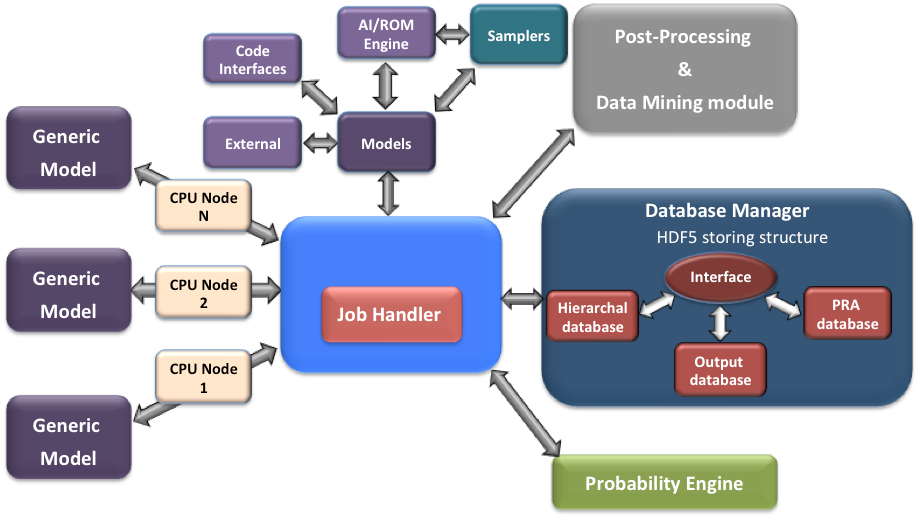
\includegraphics[width=1.0\textwidth]  {pics/RavenFramework.png}
  \caption{RAVEN framework layout}
  \label{fig:RAVENframeworkLayout}
\end{figure}

Hence, RAVEN is coded in $Python$ and is characterized by an object-oriented design. The core of the analysis performable through RAVEN is represented by a set of basic components (objects) the user can combine, in order to create a custom analysis flow. A list of these components and a summary of their most important functionalities are reported as follows:
\begin{itemize}
\item	Distribution: In order to explore the input/output space, RAVEN requires the capability to perturb the input space (initial conditions and/or model coefficients of a system code). The input space is generally characterized by probability distribution functions (PDFs), which might need to be considered when a perturbation is applied. In this respect, a large library of PDFs is available.
\item Sampler: A proper approach to sample the input space is fundamental for the optimization of the computational time. In RAVEN, a ``sampler'' employs a unique perturbation strategy that is applied to the input space of a system. The input space is defined through the connection of uncertain variables and their relative probability distributions.
\item Model: A model is the representation of a physical system (e.g. Nuclear Power Plant); it is therefore capable of predicting the evolution of a system given a coordinate set in the input space. In addition it can represent an
action on a data in order to extract key features (e.g. Data mining).
\item Reduced Order Model (ROM): The evaluation of the system response, as a function of the coordinates in the input space, is very computationally expensive, especially when brute-force approaches (e.g. Monte Carlo methods) are chosen as the sampling strategy. ROMs are used to lower this cost, reducing the number of needed points and prioritizing the area of the input space that needs to be explored. They can be considered as an artificial representation of the link between the input and output spaces for a particular system.
\end{itemize}
The list above is not comprehensive of all the RAVEN framework components (visualization and storage infrastructure).
\\ Figure~\ref{fig:RAVENframeworkLayout} shows a schematic representation of the whole framework, highlighting the communication pipes among the different modules and engines. As can be seen, in the figure all the components reported above are schematically shown. In addition the data management, mining and processing modules are shown.

\subsubsection{Distribution}
As already mentioned, the perturbation of the input space, through the initial conditions (parameters) affected by uncertainties, needs to be performed by the proper distribution functions. RAVEN provides, through an interface to the BOOST library, the following variate (truncated and not) distributions: Bernoulli, Binomial, Exponential, Logistic, Lognormal, Normal, Poisson, Triangular, Uniform, Weibull, Gamma, and Beta.
\\The usage of uni-variate distributions for sampling initial conditions is based on the assumption that the uncertain parameters are not correlated with each other. Quite often uncertain parameters are subject to correlations and thus the uni-variate approach is not applicable. This happens when a generic outcome is dependent on different phenomena simultaneously (i.e. the outcome dependency description can not be collapsed to a function of a single variable). RAVEN currently supports both N-dimensional (N-D) PDFs. The user can provide the distribution values on either Cartesian or sparse grid, which determines the interpolation algorithm used in the evaluation of the imported CDF/PDF:
\begin{enumerate}
\item N-Dimensional Spline, for Cartesian grids
\item Inverse weight, for sparse grids
\end{enumerate}
Internally, RAVEN provides the needed N-D differentiation and integration algorithms to compute the PDF from the CDF and vice-versa.
\\As already mentioned, the sampling methods use the distributions in order to perform probability-weighted perturbations. For example, in the Monte Carlo approach, a random number $\in [0,1]$ is generated (probability threshold) and the CDF, corresponding to that probability, is inverted in order to retrieve the parameter value usable in the simulation. The existence of the inverse for variate distributions is guaranteed by the monotonicity of the CDF. For N-D distributions this condition is not sufficient since the $CDF(X)\longrightarrow [0,1],X \in  R^{N} $ and therefore it could not be a bijective function. From an application point of view, this means the inverse of a N-D CDF is not unique.
\\As an example, the Figure~\ref{fig:NDDistributionExample} shows a multivariate normal distribution for a pipe failure as function of the pressure and temperature. The plane identifies an isoprobability surface (in this case, a line) that represents a probability threshold of 50 \% in this example.  Hence, the inverse of this CDF is an infinite number of points.
 \\As easily inferable, the standard sampling approach cannot directly be employed. When multivariate distributions are used, RAVEN implements a surface search algorithm for identifying the iso-probability surface location. Once the location of the surface has been found, RAVEN chooses, randomly, one point on it.

\begin{figure}
  \centering
  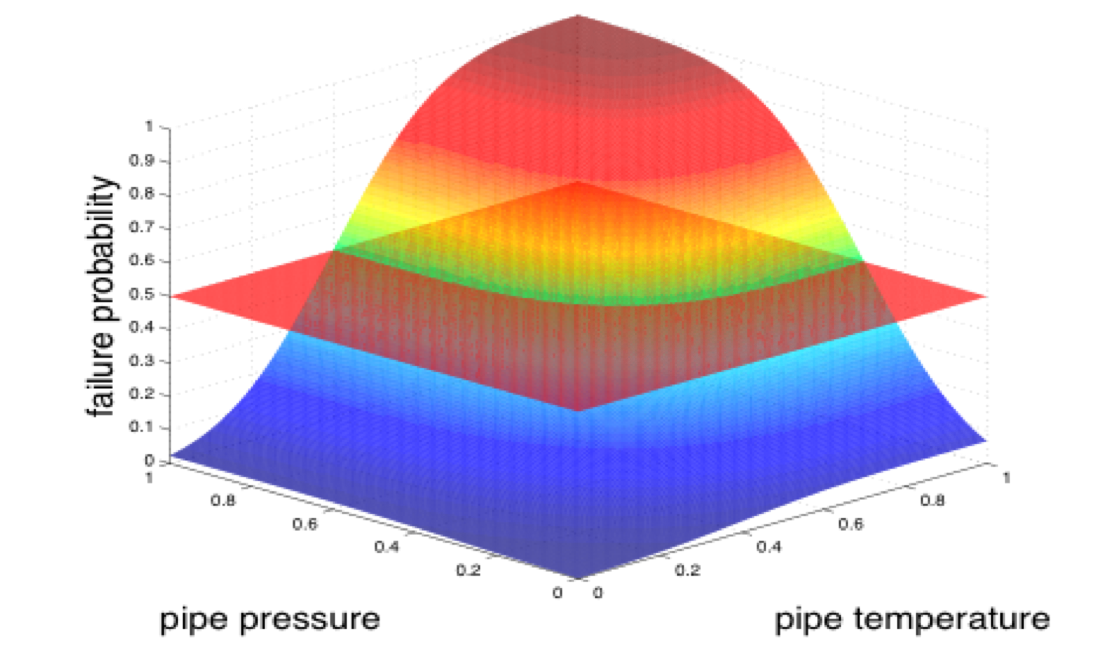
\includegraphics[width=0.5\textwidth]  {pics/NDimensionalDistributionExample.png}
  \caption{2-D CDF, function of pressure and temperature}
  \label{fig:NDDistributionExample}
\end{figure}

\subsubsection{Sampler}

The sampler is probably the most important entity in the RAVEN framework. Indeed, it performs the driving of the specific sampling strategy and, hence, determines the effectiveness of the analysis, from both an accuracy and computational point of view.  The samplers, that are available in RAVEN, can be categorized in three main classes:
\begin{itemize}
 \item Forward
 \item Dynamic Event Tree (DET)
 \item Adaptive
\end{itemize}
\paragraph{Forward Samplers} ~\\
The Forward sampler category collects all the strategies that perform the sampling of the input space without exploiting, through dynamic learning approaches, the information made available from the outcomes of calculation previously performed (adaptive sampling) and the common system evolution (patterns) that different sampled calculations can generate in the phase space (dynamic event tree).
In the RAVEN framework, several different and well-known forward samplers are available:
\begin{itemize}
\item Monte Carlo (MC)
\item Stratified based, whose most known specialization is the Latin Hyper-Cube Sampling (LHS)
\item Grid Based
\item Response Surface Design of Experiment
\item Sparse Grid
\item Factorials
\item Etc.
\end{itemize}
As already mentioned, all these sampling strategies are well known, as well as their properties. Therefore, a detailed investigation of their application is not provided.
%%%%%%%%%%%%%%%%%%%%%%%%%%%%%%%%%%%%%%%%%%%%%%%%%%%%%%%%%%%%%%%%%%%%%%%%%%%%%%%%
\paragraph{Dynamic Event Tree Samplers}~\\
In order to clarify the idea behind the Dynamic Event Tree Sampler currently available in RAVEN, a small overview is needed.
\\In technological complex systems, as nuclear power plants, an accident scenario begins with an initiating event and then evolves over time through the interaction of dynamics and stochastic events. This mutual action leads to the production of infinitely many different scenarios, which define a continuous dynamic event tree with infinite branches. At each time point, the stochastic variability of the accident outcomes is determined by a multivariate probability distribution. The PRA analysis needs an approximation to this distribution for selected consequence variables. A way to achieve this goal is an Event Tree approach. In dynamic PRA analysis, Conventional Event Tree sequences are run simultaneously starting from a single initiating event. The branches occur at user specified times and/or when an action is required by the operator and/or the system, creating a deterministic sequence of events based on the time of their occurrence. One of the disadvantages of this method is that the timing/sequencing of events and system dynamics is not explicitly accounted for in the analysis. In order to overcome these limitations a “dynamic” approach is needed. The Dynamic Event Tree (DET) technique brings several advantages, among which is the fact that it simulates probabilistic system evolution in a way that is consistent with the severe accident model. This leads to a more realistic and mechanistically consistent analysis of the system taken into consideration. The dynamic PRA, in general, and the Dynamic Event Tree methodologies in particular, are designed to take the timing of events explicitly into account, which can become very important especially when uncertainties in complex phenomena are considered. Hence, the main idea of this methodology is to let a system code determine the pathway of an accident scenario.
\\From an application point of view, a N-D grid is built on the CDF space. A single simulation is spawned and a set of triggers is added to the system code control logic. Every time a trigger gets activated (one of the CDF thresholds in the grid is violated), a new set of simulations (branches) is spawned. Each branch carries its own probability.
\\Figure \ref{fig:DETschemeExample} shows a practical example. In this particular case, it is assumed that the
probability failure of a pipe depends on the fluid pressure magnitude. Three probability thresholds are defined on
the cumulative distribution function. One simulation is spawned (0). As soon as the pressure of the fluid reaches a
value corresponding to a 33\% probability (CDF), a stop signal is sent and the framework starts two new
simulations (branches). The branch in which the system evolved to the newer condition (pipe failed, red line)
carries 33\% of the probability, while the other the complementary amount. The same procedure is repeated at
point 2.
\\Generally, not all the input space can be explored using a DET approach. For instance, usually the parameters affected by aleatory uncertainty are sampled using a dynamic event tree approach, while the ones characterized by epistemic uncertainty are sampled through ``forward'' sampling strategies.
\\As already mentioned, this strategy requires a tight interaction between the system code and the sampling driver (i.e., RAVEN framework). In addition, the system code must have a control logic capability (i.e. trigger system). For these reasons, the application of this sampling approach to a generic code needs a larger effort when compared to the other Samplers available in RAVEN. Currently, the DET is fully available for the thermal-hydraulic codes RELAP-7 and RELAP5-3D.
\\In the RAVEN framework, several different DET-based samplers are available:
\begin{itemize}
\item Dynamic Event Tree (aleatory sampling);
\item Hybrid Dynamic Event Tree (aleatory and epistemic sampling);
\item Adaptive Dynamic Event Tree (goal-oriented sampling for aleatory sampling);
\item Adaptive Hybrid Dynamic Event Tree (goal-oriented sampling for aleatory and epistemic sampling).
\end{itemize}

\begin{figure}
  \centering
  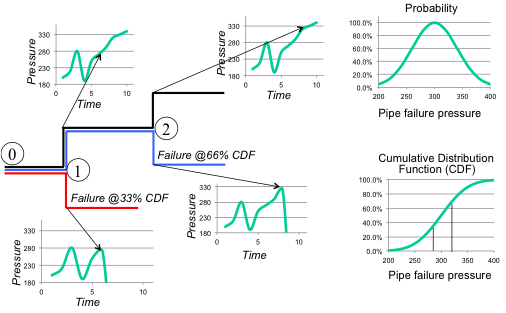
\includegraphics[width=0.7\textwidth]  {pics/DETscheme.png}
  \caption{Dynamic Event Tree simulation pattern}
  \label{fig:DETschemeExample}
\end{figure}

%%%%%%%%%%%%%%%%%%%%%%%%%%%%%%%%%%%%%%%%%%%%%%%%%%%%%%%%%%%%%%%%%%%%%%%%%%%%%%%%
\paragraph{Adaptive Samplers}~\\
A key feature available within RAVEN is the possibility to perform smart sampling (also known as adaptive sampling) as an alternative to classical ``forward'' techniques.
\\The motivation is that nuclear simulations are often computationally expensive, time-consuming, and high dimensional with respect to the number of input parameters. Thus, exploring the space of all possible simulation outcomes is unfeasible using finite computing resources. During simulation-based probabilistic risk analysis, it is important to discover the relationship between a potentially large number of input parameters and the output of a simulation using as few simulation trials as possible.
\\This is a typical context for performing adaptive sampling where a few observations are obtained from the simulation, a reduced order model (ROM) is built to represent the simulation space, and new samples are selected based on the model constructed. The ROM is then updated based on the simulation results of the sampled points. In this way, it is attempted to gain the most information possible with a small number of carefully selected sampled points, limiting the number of expensive trials needed to understand features of the system space.
\\In the RAVEN framework, several different adaptive samplers are available:
\begin{itemize}
\item Limit Surface Search;
\item Adaptive Dynamic Event Tree;
\item Adaptive Hybrid Dynamic Event Tree ;
\item Adaptive Sparse Grid;
\item Adaptive Sobol Decomposition.
\end{itemize}

\subsubsection{Models}
The Model entity, in the RAVEN environment, represents a ``connection pipeline'' between the input and the output space. The RAVEN framework does not own any physical model (i.e. it does not posses the equations needed to simulate a generic physical system, such as Navier-Stocks equations, Maxwell equations, etc.), but implements Application Program Interfaces (APIs) by which any generic model can be integrated and interrogated. The RAVEN framework provides APIs for four different model categories: Codes, Externals, Post-Processors (PPs) and Reduced Order Models (ROMs). In the following paragraphs, a brief explanation of each of this Model categories is reported.
\paragraph{Code} ~\\
The \textit{Code} model represents the communication pipe between the RAVEN framework and any system and physical code. The communication between RAVEN and any driven code is performed through the implementation of interfaces directly operated by the framework.
\\The procedure of coupling a new code/application with RAVEN is a straightforward process. The coupling is performed through a \textit{Python}  interface that interprets the information coming from RAVEN and translates them to the input of the driven code. The coupling procedure does not require modifying RAVEN itself. Instead, the developer creates a new \textit{Python} interface that is going to be embedded in RAVEN at run-time (no need to introduce hard-coded coupling statements).  This interface needs to be placed in a folder (whatever name) located in (see figure~\ref{fig:CodeInterfaceLocation}):
\begin{lstlisting}[language=bash]
 path/to/raven/distribution/raven/framework/CodeInterfaces/
\end{lstlisting}

\begin{figure}
  \centering
  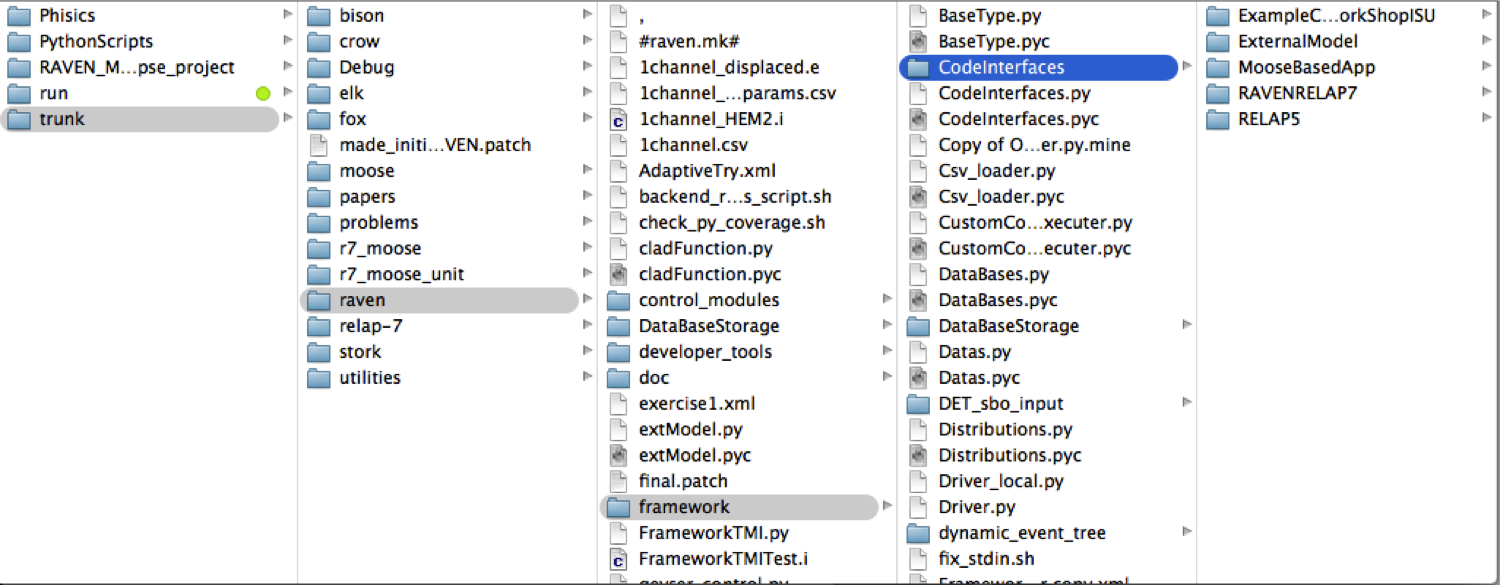
\includegraphics[width=0.8\textwidth]  {pics/CodeInterfaceLocation.png}
  \caption{Code Interface Location}
  \label{fig:CodeInterfaceLocation}
\end{figure}
At the initialization stage, RAVEN imports all the Interfaces that are contained in this directory and performs some preliminary cross-checks.
\\ If the coupled code is parallelized and/or multi-threaded, RAVEN is going to manage the system in order to optimize the computational resources in both workstations and High Performance Computing systems.
\\Currently, RAVEN has APIs for RELAP5-3D, RELAP-7, any MOOSE-based application, SASS and Modelica.
\paragraph{External Model} ~\\
The External model allows the user to create, in a \textit{Python} file (imported, at run-time, in the RAVEN framework), its own model (e.g. set of equations representing a physical model, connection to another code, control logic, etc.). This model will be interpreted/used by the framework and, at run-time, will become part of RAVEN itself.
\paragraph{Post-Processor} ~\\
The Post-Processor model represents the container of all the post-processing capabilities in the RAVEN code. This model is aimed to process the data (for example, derived from the sampling of a physical code) in order to identify representative Figure of Merits. This system has  been designed and, presently, is under heavy development by the whole RAVEN team.  Currently, the following post-processors are available:
\begin{itemize}
 \item \textit{Basic Statistics}, container of the algorithms to compute many of the most important statistical quantities. This post-processor is able to compute mean, sigma/variance, variation coefficient, skewness, kurtosis, median, percentiles and all the principal matrix quantities such as covariance, sensitivity (either leas-squared and variance weighted) and correlation matrices;
 \item \textit{Comparison Statistics}, aimed to employ validation and verification metrics;
 \item \textit{Limit Surface}, aimed to compute the limit surface in the input space (i.e. the hyper-surface that represents the boundary between the failure/success of the system);
 \item \textit{Limit Surface Integral}, intended to compute the integral of the limit surface that corresponds to the probability of failure;
  \item \textit{Safest Point}, provides the coordinates of the farthest point from the limit surface that is given as an input. The safest point coordinates are expected values of the coordinates of the farthest points from the limit surface in the space of the ``controllable'' variables based on the probability distributions of the ``non-controllable'' variables. The term ``controllable'' identifies those variables that are under control during the system operation, while the ``non-controllable'' variables are stochastic parameters affecting the system behavior randomly;
 \item \textit{External Post-Processor}, user-defined post-processor;
 \item \textit{Topological Decomposition}, aimed to compute an approximated hierarchical Morse-Smale complex which will add two columns to a data-set, performing a topological decomposition of such data-set;
 \item \textit{Data Mining}, container of all the RAVEN data mining, clustering and dimensionality reduction techniques aimed to identify dominant and common patterns in high-dimensionality data.
\end{itemize}
\paragraph{Reduced Order Model} ~\\
 As briefly mentioned, a ROM is a mathematical representation of a system, used to predict a selected output space of a physical system.
The ``training'' is a process that uses sampling of the physical model to improve the prediction capability (capability to predict the status of the system given a realization of the input space) of the ROM. More specifically, in RAVEN the Reduced Order Model is trained to emulate a high fidelity numerical representation (system codes) of the physical system. Two general characteristics of these models can be generally assumed (even if exceptions are possible):
\begin{enumerate}
   \item The higher the number of realizations in the training sets, the higher is the accuracy of the prediction performed by the reduced order model. This statement is true for most of the cases although some ROMs might be subject to the over-fitting issues. The over-fitting phenomenon is not discussed here, since its occurrence is highly dependent on the algorithm type, (and there is large number of ROM options available in RAVEN). Every time the user chooses a particular reduced order model algorithm to use, he should consult the relative literature;
   \item The smaller the size of the input domain with respect to the variability of the system response, the more likely the surrogate model will be able to represent the system output space.
\end{enumerate}
In most of the cases of interest, the information that is sought is related to defining the failure boundaries of a system with respect to perturbations in the input space. For this reason, in the development of RAVEN, it has been given priority to the introduction of a class of supervised learning algorithms, which are usually referred to as classifiers. A classifier is a reduced order model that is capable of representing the system behavior through a binary response (failure/success).
\\The first class of classifier introduced has been the Support Vector Machines (SVMs) [reference] with several different kernels (polynomial of arbitrary integer order, radial basis function kernel, sigmoid) followed by a nearest-neighbor based classification using a K-D tree search algorithm. Currently, RAVEN supports around 40 different ROM methodologies. All these supervised learning algorithms have been imported via an API from the scikit-learn [reference] library. In addition, the N-Dimensional spline and the inverse weight methods, that are currently available for the interpolation of N-Dimensional PDF/CDF, can also be used as ROMs.
\subsubsection{Simulation Environment}
RAVEN is perceived by the user as a pool of tools and data. Any action in which the tools are applied to the data is considered a calculation ``step'' in the RAVEN environment. Simplistically, a ``step'' can be seen as a \textbf{transfer function} between the input and output space through a Model (e.g. Code, External, ROM or Post-Processor). One of the most important step in the RAVEN framework is called ``multi-run'', that is aimed to handle calculations that involve multiple runs of a driven code (sampling strategies). Firstly, the RAVEN input file associates the variables to a set of PDFs and to a sampling strategy. The ``multi-run'' step is used to perform several runs in a block of a model (e.g. in a MC sampling).
\begin{figure}[ht]
  \centering
  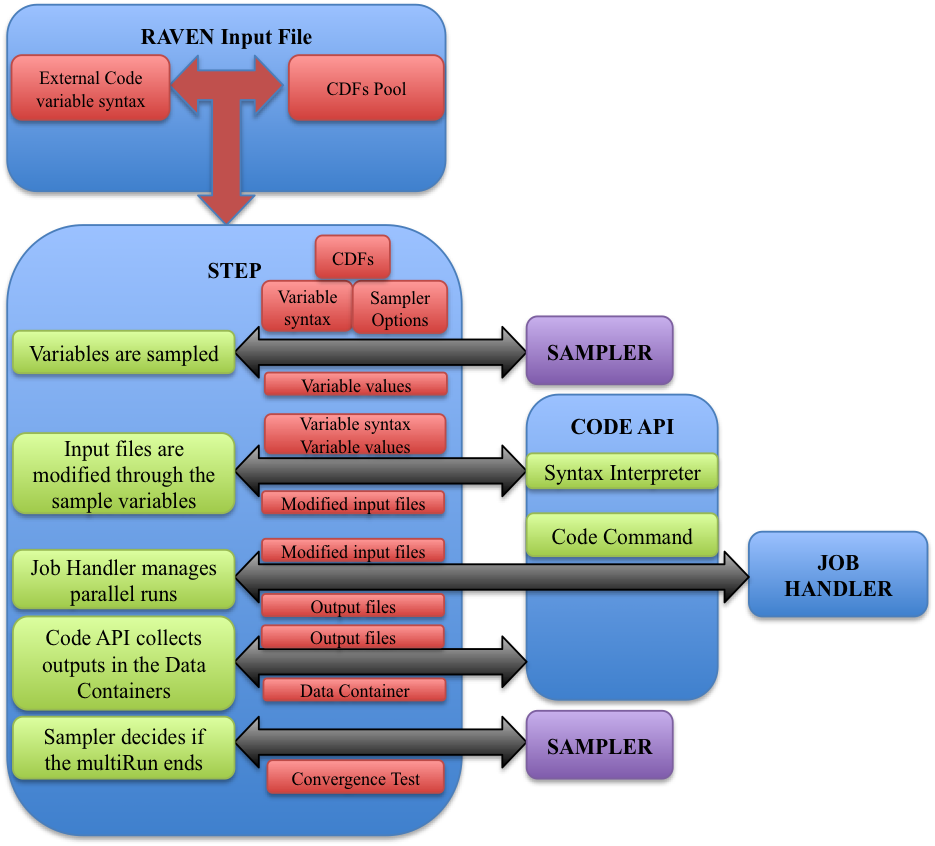
\includegraphics[width=0.8\textwidth]  {pics/MultiRunCalculationFlow.png}
  \caption{Calculation flow for a multi-run sampling}
  \label{fig:multiRun}
\end{figure}
At the beginning of each sub sequential run, the sampler provides the new values of the variables to be perturbed. The code API places those values in the input file. At this point, the code API generates the run command and asks to be queued by the job handler. The job handler manages the parallel execution of as many runs as possible within a user prescribed range and communicates with the step controller when a new set of output files are ready to be processed. The code API receives the new input files and collects the data in the RAVEN internal format. The sampler is queried to assess if the sequence of runs is ended, if not, the step controller asks for a new set of values from the sampler and the sequence is restarted as described in Figure~\ref{fig:multiRun}.
The job handler is currently capable to run different run instances of the code in parallel and can also handle codes that are multi-threaded or using any form of parallel implementation.
RAVEN also has the capability to plot the simulation outcomes while the set of sampling is performed and to store the data for later recovery.

\section{RAVEN Mathematical Background}
\label{sec:mathBackground}
\subsection{System and Control Model}
\label{sub:controlAndSystem}
The first step is the derivation of the mathematical model representing, with a high
level of abstraction, the plant and control system model. Let $\overline{\theta}\left ( t
\right )$ be a vector describing the system status in the phase space, characterized
by the following governing equation:
\begin{equation}
\label{eq:dThetaOverDT}
\frac{\partial \overline{\theta} }{\partial t}=\overline{H}\left (  \overline{\theta}\left ( t \right ),t \right )
\end{equation}
In Equation above, the assumption of time differentiability of the trajectory equation $\overline{H}\left (  \overline{\theta}\left ( t \right ),t \right )$ in the phase space has been taken. This assumption is not fully correct and generally required and it is used here, without missing of generality, for compactness of the notation.
\\It can now be performed an arbitrary decomposition of the phase space:
\begin{equation}
\label{eq:thetaDecomposition}
  \overline{\theta} = \left (\frac{\overline{x}}{\overline{v}}  \right )
\end{equation}
The decomposition is made in such a way that $\overline{x}$ represent the unknowns
solved by a system code (such as RELAP5-3D~\cite{RELAP5userManual},
RELAP7~\cite{relap7FY12}, etc.) while $\overline{v}$ are the variables directly
controlled by the control system (e.g., automatic mitigation systems, operator actions,
etc.).
\\The governing equation can be now cast in the following system of equations:
\begin{equation}
\label{eq:governingEquations}
\left\{\begin{matrix}
\frac{\partial \overline{x} }{\partial t} = \overline{F}\left (  \overline{x}, \overline{v}, t \right )  \\
\frac{\partial \overline{v} }{\partial t} = \overline{V}\left (  \overline{x}, \overline{v}, t \right )
\end{matrix}\right.
\end{equation}
Consequentially to this splitting, $\overline{x}$ contains the state variables of the
phase space that are continuous while $\overline{v}$ contains discrete state
variables that are usually handled by the control system (consequentially, named
\textbf{control variables}). It can be noticed that the
function  $ \overline{V}\left (  \overline{x}, \overline{v}, t \right )$, representing the
control system, does not depend on the  knowledge of the complete status of the
system but on a restricted subset that can be named \textbf{monitored variables} $\overline{C}$:

\begin{equation}
\label{eq:controlVars}
\left\{\begin{matrix}
\frac{\partial \overline{x} }{\partial t} = \overline{F}\left (  \overline{x}, \overline{v}, t \right )  \\
 \overline{C} =  \overline{G}(\overline{x},t)     \\
\frac{\partial \overline{v} }{\partial t} = \overline{V}\left (  \overline{x}, \overline{v}, t \right )
\end{matrix}\right.
\end{equation}
where $\overline{C}$ is a vector of smaller dimensionality than $\overline{x}$ and,
therefore, more convenient to handle.
\\As it can be noticed, the standard nomenclature of \textit{signals} (monitored variables) and \textit{status} (control variables) is not adopted. Two principal reasons
justify this decision:
\begin{itemize}
  \item The definition of signals is tight to the definition of the
  control logic for each component and, therefore, relative rather than absolute in the
  overall system analysis. For example, it is possible the the \textit{signals} for a
  component represent \textit{status} of another one, determining an in-unique
  definition.
  \item The standard nomenclature becomes meaningless when this derivation is
  applied to Uncertainty Quantification (UQ).
\end{itemize}

\subsubsection{Splitting Approach for the Simulation of the Control System}
Equation~\ref{eq:controlVars} represents a fully coupled system of Partial Differential
Equations (PDEs). To solve this system, an  \textit{operator splitting} approach
is employed. This method is preferable in this context for several reasons, among which the following:
\begin{itemize}
  \item In reality, the control system (automatic mitigation systems, operator actions,
  etc.) is always characterized by an intrinsic delay
  \item The reaction of the control system might make the system ``move'' among
  different discrete states; therefore, numerical errors will be always of first order
  unless the discontinuity is explicitly treated.
\end{itemize}
Employing the \textit{operator splitting} approach, Equation ~\ref{eq:controlVars}  can be
cast as follows:
\begin{equation}
\label{eq:operatorSplitting}
\left\{\begin{matrix}
\frac{\partial \overline{x} }{\partial t} = \overline{F}\left (  \overline{x},\overline{v}_{t_{i-1}}, t \right )  & \\
\overline{C} =  \overline{G}(\overline{x},t)  & t_{i-1} \leq t \leq  t_{i} =  t_{i-1} + \Delta  t_{i}\\
\frac{\partial \overline{v} }{\partial t} = \overline{V}\left (  \overline{x}, \overline{v}_{t_{i-1}}, t \right ) &
\end{matrix}\right.
\end{equation}
Hence, the system of equations in solved decomposing it into simpler sub-problems that are treated individually
using specialized numerical algorithms.

\subsubsection{Definition of the Monitored Variable Space}
The contraction of the information from the $\overline{x}$ space to the $\overline{C}$ space is a crucial step.
Since $\overline{C}$ represents an arbitrary middle step, it is needed to define a set of rules that make this
choice unique. $\overline{C}$ is chosen such that:
\begin{itemize}
  \item The solution of  $ \left.\begin{matrix} \frac{\partial \overline{v} }{\partial t}
  \end{matrix}\right| =\overline{V}\left (  \overline{x},\overline{v}_{t_{i-1}}, t \right )$
  can be carried along without any knowledge of the solution algorithm of
   $ \left.\begin{matrix}
  \frac{\partial \overline{x} }{\partial t} =  \end{matrix}\right| \overline{F}\left (
  \overline{x},\overline{v}_{t_{i-1}}, t \right )
  $. This requirement determines the minimum information contraction from  $\overline{x}$ to
  $\overline{C}$.
  \item All actions represented by $\overline{C} = \overline{G}(\overline{x},t)$ require knowledge of the
  solution algorithm of
  $ \left.\begin{matrix}
  \frac{\partial \overline{x} }{\partial t} =  \end{matrix}\right| \overline{F}\left (
  \overline{x},\overline{v}_{t_{i-1}}, t \right )  $. This requirement determines  the maximum  information contraction from  $\overline{x}$ to  $\overline{C}$.
\end{itemize}
The intersection of the two sub-spaces defined above create a minimal unique set.
\subsubsection{Definition of the Auxiliary Variable Space}
In the previous sections, it has been determined that the needed information to model the dynamic system
is contained in the solution vectors $\overline{x}$ and $\overline{v}$. Even if $\overline{x}$ and $\overline{v}$
are sufficient to assess the system status at every point in time, it can result in an unpractical way to model
the eventual control system.
Let's suppose to model a component of a particular system that presents different behavior depending on
other systems or operation behaviors. In order to define the status of this component in every point in time, the
whole history of the system needs to be tracked. In order to remove these inefficiency, a set of auxiliary variables
$\overline{a}$ can be introduced. These variables are the ones that in the analysis of stochastic dynamics
are artificially added into the phase space to a non-Markovian system to obtain back a Markovian behavior. In this
way only the previous time-step information is needed to determine the status of the system.
\\ Adding this additional system of variables, Equation ~\ref{eq:operatorSplitting} can be casted as follows:

\begin{equation}
\label{eq:auxiliaryVariables}
\left\{\begin{matrix}
\frac{\partial \overline{x} }{\partial t} = \overline{F}\left (  \overline{x},\overline{v}_{t_{i-1}}, t \right )  & \\
\overline{C} =  \overline{G}(\overline{x},t)  & t_{i-1} \leq t \leq  t_{i} =  t_{i-1} + \Delta  t_{i}\: \\
\frac{\partial \overline{a} }{\partial t} = \overline{A}\left (  \overline{x},\overline{C},\overline{a},\overline{v}_{t_{i-1}}, t \right ) \\
\frac{\partial \overline{v} }{\partial t} = \overline{V}\left (  \overline{C},\overline{a}, \overline{v}_{t_{i-1}}, t \right )  &
\end{matrix}\right.
\end{equation}

\subsection{Dynamic Systems Stochastic Modeling}
%
\subsubsection{General system of equations and variable classification}
\label{subsub:generalSystemOfEqAndVarsClassification}
In Section ~\ref{sub:controlAndSystem}, the derivation of the governing equations for a controllable system
have been reported. In this section, the mathematical framework of the modeling of dynamic stochastic systems,
under uncertainties, is derived.
\\ Dynamic stochastic systems are the ones whose dynamic is characterized by intrinsic randomness. Random
behaviors, although present in nature, are often artificially introduced into physical models to account for the
incapability of fully modeling part of the nature of the system behavior and/or of the phenomena bounding the
physical problem.
\\The distinction between variables that are artificially considered aleatory and the ones intrinsically aleatory
corresponds with the classical definition of epistemic and aleatory uncertainties. From a
system simulation point of view it is more relevant how these variables, the sources of aleatory behavior, change
in time.
Possible examples of random elements are:
\begin{itemize}
 \item random variability of parameters (e.g., uncertainty in physical parameters)
 \item presence of noise (background noise due to intrinsically stochastic behaviors or lack of detail in the
 simulation)
 \item Uncertainty in the initial and boundary conditions
 \item Random failure of components
 \item aging effects.
\end{itemize}
Before introducing the mathematical models for uncertainty,  it can beneficial to recall
Equation ~\ref{eq:dThetaOverDT}, adding the initial conditions:
\begin{equation}
\label{eq:dThetaOverDTWithBoundary}
\left\{\begin{matrix}
\frac{\partial  \overline{\theta}\left ( t \right )}{\partial t}=\overline{H}\left (  \overline{\theta}\left ( t \right ),t \right ) \\
 \overline{\theta}\left ( t_{0} \right ) = \overline{\theta}_{0}
\end{matrix}\right.
\end{equation}
At this point, each source of uncertainty or stochastic behavior is considered and progressively added in
Equation ~\ref{eq:dThetaOverDTWithBoundary}.
For the scope of this derivation, it is convenient to split the phase space into \textit{continuous} (e.g.,temperature,
pressure, hentalpy, etc.) and discrete (e.g.,status of components, such as operational and failure states) variables
as follows:
\begin{itemize}
 \item $ \overline{\theta}^{c} \in \Phi \subseteq \mathbb{R}^{C}$, the set of continuous variables
 \item $ \overline{\theta}^{d} \in \Psi \subseteq \mathbb{N}^{D}$, the set of discrete variables
 \item $\overline{\theta}(t) = \overline{\theta}^{c} \oplus \overline{\theta}^{d}$.
\end{itemize}
Consequentially, Equation ~\ref{eq:dThetaOverDTWithBoundary} assumes the following form:
\begin{equation}
\label{eq:systemThetaContAndDescrete}
\left\{\begin{matrix}
\frac{\partial  \overline{\theta}^{c}\left ( t \right )}{\partial t}=f\left ( \overline{\theta}^{c},\overline{\theta}^{d},t \right ) \\
\frac{\partial  \overline{\theta}^{d}\left ( t \right )}{\partial t}=g\left ( \overline{\theta}^{c},\overline{\theta}^{d},t \right )\\
 \overline{\theta}^{c}\left ( t_{0} \right ) = \overline{\theta}^{c}_{0}\\
 \overline{\theta}^{d}\left ( t_{0} \right ) = \overline{\theta}^{d}_{0}
\end{matrix}\right.
\end{equation}
Note that the time derivative operator has been also used for the time discontinuous variables, even
if this is allowed only introducing complex extension of the time derivative operator. In this context, the $\frac{\partial  }{\partial t}$ on the discontinuous space is employed for simplifying the notation only.

\subsubsection{Probabilistic Nature of the Parameters Characterizing the Equation}
As shown in Equation ~\ref{eq:systemThetaContAndDescreteStaz}, The first stochastic behaviors to be introduced are the
uncertainties associated with the:
\begin{itemize}
  \item initial conditions (i.e. $\overline{\theta}^{c}$ and $\overline{\theta}^{d}$ at time $t_{0}$), and
  \item parameters characteristic of  $f\left ( \overline{\theta}^{c},\overline{\theta}^{d},t \right )$ and $g\left ( \overline{\theta}^{c},\overline{\theta}^{d},t \right )$.
\end{itemize}

\begin{equation}
\label{eq:systemThetaContAndDescreteStaz}
\left\{\begin{matrix}
\frac{\partial  \overline{\theta}^{c}\left ( t \right )}{\partial t}=f\left ( \overline{\theta}^{c},\overline{\theta}^{d}, \overline{\alpha}_{staz} ,      t \right ) \\
\frac{\partial  \overline{\theta}^{d}\left ( t \right )}{\partial t}=g\left ( \overline{\theta}^{c},\overline{\theta}^{d},\overline{\alpha}_{staz},t \right )\\
\Pi \left ( \overline{\theta}^{c},t_{0} \right ) \sim pdf\left ( \overline{\theta}^{c}_{0}|,\sigma_{c}^{2} \right )\\
\Pi \left ( \overline{\theta}^{d},t_{0} \right ) \sim pdf\left ( \overline{\theta}^{d}_{0}|,\sigma_{d}^{2} \right ) \\
\overline{\alpha}_{staz}\left ( t \right )=\overline{\alpha}_{staz}\left ( t_{0} \right ) \sim pdf\left ( \overline{\alpha}_{staz}^{0}|, \sigma_{staz}^{2} \right )
\end{matrix}\right.
\end{equation}
In Equation ~\ref{eq:systemThetaContAndDescreteStaz}, $\Pi \left ( \overline{\theta}^{c},t_{0} \right )$ indicates the
probability distribution of $\overline{\theta}^{c}$ at the initial time $t=t_{0}$ while
$pdf\left ( \mu|, \sigma^{2} \right )$ represents a generic probability distribution function having mean value
$\mu$ and sigma $\sigma$.The term $\overline{\alpha}_{staz}$ is the vector of parameters affected by
uncertainty but not varying over time.
\\As already mentioned, Equation ~\ref{eq:systemThetaContAndDescreteStaz} considers uncertainties whose values
do not change during the dynamic evolution of the system. This set of uncertainties accounts for most of the
common source of aleatory behaviors. Examples of this kind of uncertainties are:
\begin{itemize}
  \item \textit{Uncertainty associated with the heat conduction coefficient}:  This value is known (but uncertain) and has no physical reason to change during the simulation;
  \item \textit{Uncertainty on failure temperature for a pipe}: This value is usually characterized by a probability distribution function but once the value has been set (like through random sampling) it will not change during the simulation.
\end{itemize}
From a modeling perspective, all the probabilistic behaviors connected to $\Pi \left ( \overline{\theta}^{c},t_{0}
\right ) $, $\Pi \left ( \overline{\theta}^{d},t_{0} \right )$ and $\overline{\alpha}_{staz}(t)$ can be modeled without
changing the dimensionality of the phase space (hence, no alteration of the solution algorithm is required), simply performing sampling of the input space. In addition, the Markovian assumption is still preserved.

\subsubsection{Variables Subject to Random Motion}
The next aleatory component to be accounted for is the set of parameters that continuously change over time (i.e. $\overline{\alpha}_{brow}$).
In other words,  these parameters are referred as if they behave like a \textit{Brownian motion}.
While what commonly is indicated as \textit{Brownian motion} has not impact at the character
the space and time scales (characteristic of a physical system), there are parameters that have (or \textbf{appear}
to have) such behavior. The  \textit{Brownian motion} characteristic of some variables can be completely
synthetic, due to the lack of modeling details in the simulation model.
\\For instance, two examples of these randomly varying variables are:
\begin{itemize}
  \item \textit{Cumulative damage growth in material}. Experimental data and models representing this
  phenomenon show large uncertainties. There is also an intrinsic natural stochasticity driving
  the accumulation of the damage (natural Brownian motion);
  \item \textit{Heat conductivity in the fuel gap during heating of fuel}. During some transients there are
  situations where the fuel is in contact with the clad while in others where there is the presence of a gap. While in
  nature this is a discontinuous transition, it is not usually possible to model in such a way, especially if vibrations
  of the fuel lead to high frequency oscillations. In this case, it would be helpful to introduce directly into the
  simulation a random noise characterizing the thermal conductivity when these transitions occur (synthetic
  Brownian motion).
\end{itemize}
The system of Equations~\ref{eq:systemThetaContAndDescreteStaz} can be rewritten in the following form:

\begin{equation}
\label{eq:systemThetaContAndDescreteStazAndBrow}
\left\{\begin{matrix}
\frac{\partial  \overline{\theta}^{c}\left ( t \right )}{\partial t}=f\left ( \overline{\theta}^{c},\overline{\theta}^{d}, \overline{\alpha}_{staz} ,\overline{\alpha}_{brow},      t \right ) \\
\frac{\partial  \overline{\theta}^{d}\left ( t \right )}{\partial t}=g\left ( \overline{\theta}^{c},\overline{\theta}^{d},\overline{\alpha}_{staz},\overline{\alpha}_{brow},t \right )\\
\frac{\partial \overline{\alpha}_{brow} }{\partial t}=b\left ( \overline{\theta}^{c},\overline{\theta}^{d},\overline{\alpha}_{staz},\overline{\alpha}_{brow},t \right )\Gamma \left ( t \right )
\\
\Pi \left ( \overline{\theta}^{c},t_{0} \right ) \sim pdf\left ( \overline{\theta}^{c}_{0}|,\sigma_{c}^{2} \right )\\
\Pi \left ( \overline{\theta}^{d},t_{0} \right ) \sim pdf\left ( \overline{\theta}^{d}_{0}|,\sigma_{d}^{2} \right ) \\
\overline{\alpha}_{staz}\left ( t \right )=\overline{\alpha}_{staz}\left ( t_{0} \right ) \sim pdf\left ( \overline{\alpha}_{staz}^{0}|, \sigma_{staz}^{2} \right ) \\
\overline{\alpha}_{brow}\left ( t_{0} \right ) \sim  \overline{\alpha}_{brow}^{0} \Gamma \left ( t_{0} \right )
\end{matrix}\right.
\end{equation}
where $\Gamma \left ( t \right )$ is 0-mean random noise and $\overline{\alpha}_{brow}$ is the set of parameters subject to \textit{Brownian motion}.
\\Clearly, the equation referring to the time change of the parameters subject to the \textit{Brownian motion} should be interpreted in the \textbf{Ito} sense [C. Gardiner, Stochastic Methods, Springer (2009)].

\subsubsection{Discontinuously and Stochastically varying variables}
The last and probably most difficult step is the introduction of parameters that are neither constant during the simulation nor continuously vary over time. As an example, consider a valve that, provided set of operating conditions, opens or closes. If this set of conditions is reached n times during the simulation, the probability of the valve correctly operating should be sampled n times. It is also foreseeable that the history of failure/success of the valve will impact future probability of failure/success.  In this case the time evolution of such parameters (discontinuously stochastic changing parameters  $\overline{\alpha}_{DS}$) is governed by the following equation:

\begin{equation}
\label{eq:systemDiscAndStochVaryVars}
\frac{\partial  \overline{\alpha }_{DS}\left ( t \right )}{\partial t}=  \overline{\delta}\left ( \overline{\alpha }_{DS}, \overline{\theta}^{c},\overline{\theta}^{d},\overline{\alpha}_{staz},\overline{\alpha}_{brow},t \right ) \times \overline{V}\left ( \overline{\alpha }_{DS}, \overline{\theta}^{c},\overline{\theta}^{d},\overline{\alpha}_{staz},\overline{\alpha}_{brow},t \right ) \times \overline{p}\left ( \int_{t_{0}}^{t}  S\left ( \overline{\theta}\left ( t^{'} \right ),t^{'} \right )dt^{'} \right )
\end{equation}
where:
\begin{itemize}
  \item The function $\overline{\delta}\left ( \overline{\alpha }_{DS}, \overline{\theta}^{c},\overline{\theta}^{d},
  \overline{\alpha}_{staz},\overline{\alpha}_{brow},t \right )$ is the delta of Dirac of the instant on which the
  transition need to be evaluated (control logic signaling to the valve to open/close).
  \item The term $\overline{p}\left ( \int_{t_{0}}^{t}  S\left ( \overline{\theta}\left ( t^{'} \right ),t^{'} \right )\right )
  = \overline{p}\left ( \int_{t_{0}}^{t}  \overline{\alpha }_{DS}, \overline{\theta}^{c},\overline{\theta}^{d},
  \overline{\alpha}_{staz},\overline{\alpha}_{brow},t dt\right )$ represents the transition probability
  between different states (in case of the valve: open/close). Note that the time integral of the
  parameter history accounts for the memory of the component via the kernel $S\left ( \overline{\theta}\left ( t^{'}
  \right ),t^{'} \right )$.
  \item The term $\overline{V}\left ( \overline{\alpha }_{DS}, \overline{\theta}^{c},\overline{\theta}^{d},
  \overline{\alpha}_{staz},\overline{\alpha}_{brow},t \right )$ is the rate of change of $\overline{\alpha }_{DS}$.
  For a discrete parameter, it is defined as the value of the instantaneous $\overline{\alpha }_{DS}$ change.
\end{itemize}
The introduction of the history dependency introduced in the term $\overline{p}$ determines that the system cannot be considered
Markovian if ``countermeasures'' are not taken. In order to make the system return to be Markovian, the phase space needs to be
expanded (i.e., increase its dimensionality): the time at which the
parameters changed status and their corresponding values $\left \{  \left (\overline{\alpha}_{DS}, t \right )_{i} \right \} = \left \{  \overline{\alpha}_{DS}, t_{i} \right \} = \overline{\overline{\alpha}}_{DS}, \overline{t}\, \left ( for\, i=1,...,n \right )$.
\\Equation~\ref{eq:systemDiscAndStochVaryVars} now assumes the form:
\begin{equation}
\label{eq:systemDiscAndStochVaryVarsExpanded}
\begin{matrix}
\frac{\partial  \overline{\alpha }_{DS}\left ( t \right )}{\partial t}=  \overline{\delta}\left ( \overline{\alpha }_{DS}, \overline{\theta}^{c},\overline{\theta}^{d},\overline{\alpha}_{staz},\overline{\alpha}_{brow},t \right ) \times \overline{V}\left ( \overline{\alpha }_{DS}, \overline{\theta}^{c},\overline{\theta}^{d},\overline{\alpha}_{staz},\overline{\alpha}_{brow},t \right ) \times \overline{p}\left ( \overline{\overline{\alpha}}_{DS},\overline{t},\overline{\theta}^{c},\overline{\theta}^{d},\overline{\alpha}_{staz},\overline{\alpha}_{brow},t  \right ) \\ \! \! \! \! \! \! \! \! \! \! \! \! \! \! \! \! \! \! \! \! \! \! \! \! \! \! \! \! \! \! \! \! \! \! \! \! \! \! \! \! \! \! \! \! \! \! \! \! \! \! \! \! \! \! \! \! \! \! \! \! \! \! \! \! \! \! \! \! \! \! \! \! \! \! \! \! \! \! \! \! \! \! \! \! \! \! \! \! \! \! \! \! \! \! \! \! \! \! \! \! \! \! \! \! \! \! \! \! \! \! \! \! \! \! \! \! \! \! \! \! \! \! \! \! \! \! \! \! \! \! \! \! \! \! \! \! \! \! \! \! \! \! \! \! \! \! \! \! \! \! \! \! \! \! \! \! \! \! \! \! \! \! \! \! \! \! \! \!
for \, t\geq t_{n}
\end{matrix}
\end{equation}
This formulation introduces a phase space that is continuously growing over time $n \rightarrow \infty$. In this respect, it is useful to introduce and discuss possible assumptions:
\begin{enumerate}
  \item The memory of the past is not affected by the time distance; in this case:
  \begin{equation}
   \overline{p}\left ( \overline{\overline{\alpha}}_{DS},\overline{t},\overline{\theta}^{c},\overline{\theta}^{d},\overline{\alpha}_{staz},\overline{\alpha}_{brow},t  \right ) =  \overline{p}\left ( \overline{\overline{\alpha}}_{DS},\overline{\theta}^{c},\overline{\theta}^{d},\overline{\alpha}_{staz},\overline{\alpha}_{brow},t  \right )
  \end{equation}
  The dimensionality of the phase space is still growing during the simulation since more and more sampling is
  performed, but the time integral is removed from the transition probability. A simple example of this situation is
  a component activated on demand in which failure is a function of all previous sampling, but not of when the
  component was sampled or in which sequence the outcome occurred.
  \item  The number of samples is determined before the simulation itself takes place (e.g.,$n$ times) In this case
  the different $\overline{\alpha}_{DS_{i}}$ could be treated explicitly as $\overline{\alpha}_{staz}$   while
  $\overline{t}$ would still remain a variable to be added to the phase space (if simplification 1 is not valid) but of
  fixed dimension. In this case $\overline{t}$ still needs to be computed and its expression is:
  \begin{equation}
   \overline{t} \left ( t \right ) = \int_{t_{0}}^{t} \overline{t}  \, \overline{\delta }\left ( \overline{\alpha }_{DS},
   \overline{\theta}^{c},\overline{\theta}^{d},\overline{\alpha}_{staz},\overline{\alpha}_{brow},t \right )  dt
  \end{equation}
  The transition probability becomes:
  \begin{equation}
     \overline{p}\left ( \int_{t_{0}}^{t} dt\, S\left ( \overline{t} \right ), \overline{\alpha}_{DS}, \overline{\theta}^{c},
     \overline{\theta}^{d},\overline{\alpha}_{staz},\overline{\alpha}_{brow},t \right )
  \end{equation}
  For example, this is the case of a component that is sampled a fixed number of times for a given simulation
  while the contribution of the history to the transition probability might decay exponentially over time. This
  approximation might eliminate the memory from the system by adding n variables to the phase space $t_{i} \, \,
  (for \, \, i=1,...,n)$ thus restoring the Markovian characteristic.
  \item Another possible approximation alternative to the previous one is that the memory of the system (here
  explicitly represented by $ \int_{t_{0}}^{t}  \overline{\alpha }_{DS} dt$) is limited
  only to a fixed number of steps back in the past. In this case $n$ is always bounded. Therefore, adding  $\left \{
  \overline{\alpha}_{DS_{i}},t_{i} \right \}, \left ( for\: i=1,...,n \right )$ would possibly preserve the system
  Markovian properties of the system. This approximation allows for eliminating the memory from the system by
  expanding the phase space $2n$ variables. From a software implementation point of view, this is the most
  complex  situation since without any simplification we would have to deal with a system that is never reducible
  to a Markovian one and therefore forced to use the whole history of the system to forecast its evolution at each
  time step.
\end{enumerate}
Assumption 1 limits this cost by restraining it to the set of values assumed by the
variable but would still lead to very difficult to deal with situation. Assumption 2 would
require an expansion of phase space to introduce the time at which the transitions
happens but the value that the parameter will assume at each sampling could be
treated as initial condition. Assumption 3 would instead require the expansion of the
phase space for both the time and the values of the
transitioning variables.
\\Based on the this simplifications, the system of
Equations~\ref{eq:systemThetaContAndDescreteStazAndBrow}, accounting also for $ \overline{\alpha}_{DS}$ can be cast into the form:
\begin{equation}
\label{eq:fullSystem}
\begin{split}
\left\{\begin{matrix}
\frac{\partial  \overline{\theta}^{c}\left ( t \right )}{\partial t}=f\left ( \overline{\theta}^{c},\overline{\theta}^{d}, \overline{\alpha}_{staz} ,\overline{\alpha}_{brow},      t \right ) \\
\frac{\partial  \overline{\theta}^{d}\left ( t \right )}{\partial t}=g\left ( \overline{\theta}^{c},\overline{\theta}^{d},\overline{\alpha}_{staz},\overline{\alpha}_{brow},t \right )\\
\frac{\partial \overline{\alpha}_{brow} }{\partial t}=b\left ( \overline{\theta}^{c},\overline{\theta}^{d},\overline{\alpha}_{staz},\overline{\alpha}_{brow},t \right )\Gamma \left ( t \right ) \\
\frac{\partial  \overline{\alpha }_{DS}\left ( t \right )}{\partial t}=  \overline{\delta}\left ( \overline{\alpha }_{DS}, \overline{\theta}^{c},\overline{\theta}^{d},\overline{\alpha}_{staz},\overline{\alpha}_{brow},t \right ) \times \overline{V}\left ( \overline{\alpha }_{DS}, \overline{\theta}^{c},\overline{\theta}^{d},\overline{\alpha}_{staz},\overline{\alpha}_{brow},t \right ) \times
\\ \times  \overline{p}\left ( \int_{t_{0}}^{t}  dt\;   \overline{\alpha }_{DS}, \overline{\theta}^{c},\overline{\theta}^{d},
  \overline{ \alpha}_{staz},\overline{\alpha}_{brow},t \right )
\\
\Pi \left ( \overline{\theta}^{c},t_{0} \right ) \sim pdf\left ( \overline{\theta}^{c}_{0}|,\sigma_{c}^{2} \right )\\
\Pi \left ( \overline{\theta}^{d},t_{0} \right ) \sim pdf\left ( \overline{\theta}^{d}_{0}|,\sigma_{d}^{2} \right ) \\
\overline{\alpha}_{staz}\left ( t \right )=\overline{\alpha}_{staz}\left ( t_{0} \right ) \sim pdf\left ( \overline{\alpha}_{staz}^{0}|, \sigma_{staz}^{2} \right ) \\
\overline{\alpha}_{brow}\left ( t_{0} \right ) \sim  \overline{\alpha}_{brow}^{0} \Gamma \left ( t_{0} \right ) \\
\overline{\alpha}_{DS} \left ( t_{0} \right ) = \overline{\alpha}_{DS} ^{0}
\end{matrix}\right.
\end{split}
\end{equation}
Introducing the Simplifications \textbf{1} and \textbf{3} ( the most
appropriated in this context), Equation ~\ref{eq:fullSystem} becomes:
\begin{equation}
\label{eq:fullSystemApprox1-3}
\begin{split}
\left\{\begin{matrix}
\frac{\partial  \overline{\theta}^{c}\left ( t \right )}{\partial t}=f\left ( \overline{\theta}^{c},\overline{\theta}^{d}, \overline{\alpha}_{staz} ,\overline{\alpha}_{brow},      t \right ) \\
\frac{\partial  \overline{\theta}^{d}\left ( t \right )}{\partial t}=g\left ( \overline{\theta}^{c},\overline{\theta}^{d},\overline{\alpha}_{staz},\overline{\alpha}_{brow},t \right )\\
\frac{\partial \overline{\alpha}_{brow} }{\partial t}=b\left ( \overline{\theta}^{c},\overline{\theta}^{d},\overline{\alpha}_{staz},\overline{\alpha}_{brow},t \right )\Gamma \left ( t \right ) \\
\frac{\partial  \overline{\alpha }_{DS}\left ( t \right )}{\partial t}=  \overline{\delta}\left ( \overline{\alpha }_{DS}, \overline{\theta}^{c},\overline{\theta}^{d},\overline{\alpha}_{staz},\overline{\alpha}_{brow},t \right ) \times \overline{V}\left ( \overline{\alpha }_{DS}, \overline{\theta}^{c},\overline{\theta}^{d},\overline{\alpha}_{staz},\overline{\alpha}_{brow},t \right ) \times
\\ \times  \overline{p}\left ( \overline{\alpha }_{DS}, \overline{\theta}^{c},\overline{\theta}^{d},\overline{\alpha}_{staz},\overline{\alpha}_{brow},t \right )
\\
\Pi \left ( \overline{\theta}^{c},t_{0} \right ) \sim pdf\left ( \overline{\theta}^{c}_{0}|,\sigma_{c}^{2} \right )\\
\Pi \left ( \overline{\theta}^{d},t_{0} \right ) \sim pdf\left ( \overline{\theta}^{d}_{0}|,\sigma_{d}^{2} \right ) \\
\overline{\alpha}_{staz}\left ( t \right )=\overline{\alpha}_{staz}\left ( t_{0} \right ) \sim pdf\left ( \overline{\alpha}_{staz}^{0}|, \sigma_{staz}^{2} \right ) \\
\overline{\alpha}_{brow}\left ( t_{0} \right ) \sim  \overline{\alpha}_{brow}^{0} \Gamma \left ( t_{0} \right ) \\
\overline{\alpha}_{DS} \left ( t_{0} \right ) = \overline{\alpha}_{DS} ^{0}
\end{matrix}\right.
\end{split}
\end{equation}
This dissertation does not cover all the possible phenomena, but it
provides a sufficient mathematical framework for extrapolating toward cases that are not explicitly treated.
\\ Given the presence of all these sources of stochastic behaviors, every
exploration of the uncertainties (through sampling strategies) only
represents a possible trajectory of the system in the phase space. Hence,
it is much more informative the assessment of the probability of a
particular response, rather than the response itself.
\\The explanation of these concepts is demanded to next section.
%
%
% Formulation of the equation set in a statistical framework
%
%
\subsection{Formulation of the equation set in a statistical framework}
Based on the premises reported in the previous sections and assuming
that at least one of the simplifications mentioned in
Section~\ref{subsub:generalSystemOfEqAndVarsClassification} is applicable (i.e. the system can be
casted as Markovian), it is needed to investigate the system evolution
in terms of its probability density function in the global phase space
$\overline{\theta}$ via the Chapman-Kolmogorov
equation~\cite{ProbReactoDynamicsDevooght}.
\\The integral form of the Chapman-Kolmogorov is the following:
\begin{equation}
\label{eq:chapKolmogIntegralForm}
\begin{matrix}
\Pi \left (\overline{\theta}_{3},t_{3}|\overline{\theta}_{1},t_{1}  \right ) = \int
d\overline{\theta}_{2} \Pi\left (\overline{\theta}_{2},t_{2}|
\overline{\theta}_{1},t_{1}  \right )   \Pi\left (\overline{\theta}_{3},t_{3}|
\overline{\theta}_{2},t_{2}  \right )   &
where \: \:   t_{1} < t_{2} < t_{3}
\end{matrix}
\end{equation}
while its differential form is:
\begin{equation}
\label{eq:chapKolmogDiffForm}
\frac{\partial \Pi \left (\overline{\theta},t|\overline{\theta}_{0},t_{0}  \right )  }{\partial t} =
\mathcal{L}_{CK}\left (   \Pi \left (\overline{\theta},t|\overline{\theta}_{0},t_{0}  \right ) \right )
\end{equation}
The transition from the integral to the differential form is possible under the following assumptions:
\begin{equation}
\label{eq:chapKolmogAssump1}
\lim_{\Delta t \to 0} \frac{1}{\Delta t}  \int_{|
\overline{\theta}_{2}-\overline{\theta}_{1}|<\varepsilon }   \Pi \left
(\overline{\theta}_{2},t+\Delta t|\overline{\theta}_{1},t  \right )
d\overline{\theta}_{2} = 0
\end{equation}

\begin{equation}
\label{eq:chapKolmogAssump2}
\lim_{\Delta t \to 0} \frac{1}{\Delta t} \Pi \left (\overline{\theta}_{2},t+\Delta t|
\overline{\theta}_{1},t  \right ) = W\left ( \overline{\theta}_{2}|
\overline{\theta}_{1},t \right )
\end{equation}

\begin{equation}
\label{eq:chapKolmogAssump3}
\lim_{\Delta t \to 0} \frac{1}{\Delta t}  \int_{|
\overline{\theta}_{2}-\overline{\theta}_{1}|<\varepsilon }
\left ( \overline{\theta}_{2,i} - \overline{\theta}_{1,i} \right )
\Pi \left (\overline{\theta}_{2},t+\Delta t|\overline{\theta}_{1},t  \right )
d\overline{\theta}_{2} = A_{i}\left ( \overline{\theta}_{1},t \right ) +
\mathcal{O}\left ( \varepsilon \right )
\end{equation}

\begin{equation}
\label{eq:chapKolmogAssump4}
\lim_{\Delta t \to 0} \frac{1}{\Delta t}  \int_{|
\overline{\theta}_{2}-\overline{\theta}_{1}|<\varepsilon }
\left ( \overline{\theta}_{2,i} - \overline{\theta}_{1,i} \right ) \left (
\overline{\theta}_{2,j} - \overline{\theta}_{1,j} \right )
\Pi \left (\overline{\theta}_{2},t+\Delta t|\overline{\theta}_{1},t  \right )
d\overline{\theta}_{2} = B_{i,j}\left ( \overline{\theta}_{1},t \right ) +
\mathcal{O}\left ( \varepsilon \right )
\end{equation}

The first condition guarantees the continuity of $\Pi \left (\overline{\theta},t|\overline{\theta}_{0},t_{0}  \right )$, while the other three force the finite existence of three parameters.
Equation 25 can be furthermore decomposed into the continuous and discrete components:

\begin{equation}
\label{eq:chapKolmogIntegralFormContDisct}
\left\{\begin{matrix}
\Pi \left (\overline{\theta}_{3}^{c},t_{3}|\overline{\theta}_{1}^{c},t_{1}  \right )
= \int \Pi \left (\overline{\theta}_{2}^{c},t_{2}|\overline{\theta}_{1}^{c},t_{1}
\right ) \Pi \left (\overline{\theta}_{3}^{c},t_{3}|\overline{\theta}_{2}^{c},t_{2}
\right ) d\overline{\theta}_{2}^{c}
\\
\Pi \left (\overline{\theta}_{3}^{d},t_{3}|\overline{\theta}_{1}^{d},t_{1}  \right )
= \int \Pi \left (\overline{\theta}_{2}^{d},t_{2}|\overline{\theta}_{1}^{d},t_{1}
\right ) \Pi \left (\overline{\theta}_{3}^{d},t_{3}|\overline{\theta}_{2}^{d},t_{2}
\right ) d\overline{\theta}_{2}^{d}
\end{matrix}\right.
\: \: \: where \:\:   t_{1}<t_{2}<t_{3}
\end{equation}

and its differential form is as follows:
\begin{equation}
\label{eq:chapKolmogDiffFormContDisct}
\left\{\begin{matrix}
\frac{\partial \Pi \left (\overline{\theta}^{c},t|\overline{\theta}_{0}^{c},t_{0}
\right ) }{\partial t} = \mathcal{L}_{CK}^{c}  \left (     \Pi \left
(\overline{\theta}^{c},t|\overline{\theta}_{0}^{c},t_{0} \right ),
\overline{\theta}^{d},\overline{\alpha}_{brow},\overline{\alpha}_{staz},
\overline{\alpha}_{DS},t  \right )
\\
\frac{\partial \Pi \left (\overline{\theta}^{d},t|\overline{\theta}_{0}^{d},t_{0}
\right ) }{\partial t} = \mathcal{L}_{CK}^{d}  \left (     \Pi \left
(\overline{\theta}^{d},t|\overline{\theta}_{0}^{d},t_{0} \right ),
\overline{\theta}^{c},t  \right )
\end{matrix}\right.
\end{equation}
where:
\begin{itemize}
 \item  $\Pi \left (\overline{\theta}^{c},t|\overline{\theta}_{0}^{c},t_{0} \right
 )$ of the system to be in state $\overline{\theta}^{c}$ at time $t$ given that
 the system was in $\overline{\theta}^{c}_{0}$ at time $t_{0}$;
 \item $\Pi \left (\overline{\theta}^{d},t|\overline{\theta}_{0}^{d},t_{0} \right
 )$ of the system to be in state $\overline{\theta}^{d}$ at time $t$ given
 that the system was in $\overline{\theta}^{d}_{0}$ at time $t_{0}$;
 \item $\mathcal{L}_{CK}^{c} \left ( \cdot  \right )$ and
 $\mathcal{L}_{CK}^{d} \left ( \cdot  \right )$  are specific Chapman-
 Kolmogorov operators that will be described in the following section.
\end{itemize}
%
%
% The Chapman-Kolmogorov Equation
%
%
% COPY FROM HERE
%
\subsection{The Chapman-Kolmogorov Equation}
\label{sec:ChapmanKolmogorov }
The system of equations~\ref{eq:thetaDecomposition}, written in integral
form, can be solved in a differential form through the Chapman-Kolmogorov (C-K)
operator~\cite{ProbReactoDynamicsDevooght}:

\begin{equation}
\label{eq:CK}
\begin{matrix}
\frac{\partial \Pi \left (\overline{\theta}^{c},t|\overline{\theta}_{0}^{c},t_{0}
\right ) }{\partial t} = - \sum_i \frac{\partial }{\partial \overline{\theta}_{i}^{c}} \left ( A_{i}\left (  \overline{\theta}^{c}, \overline{\theta}^{d}, t\right ) \Pi \left (\overline{\theta}^{c},t|\overline{\theta}_{0}^{c},t_{0}
\right )  \right ) +
\\
+ \frac{1}{2}\sum_{i,j} \frac{\partial^2 }{\partial \overline{\theta}^{c}_{i} \partial \overline{\theta}^{c}_{j}}\left ( B_{i,j}\left (  \overline{\theta}^{c}, \overline{\theta}^{d}, t\right ) \Pi \left (\overline{\theta}^{c},t|\overline{\theta}_{0}^{c},t_{0}
\right )  \right ) +
\\
+ \int \left (  W\left ( \overline{\theta}^{c}|
\overline{\theta}^{'c},\overline{\theta}^{d},t \right )\Pi \left (\overline{\theta}^{'c},t|\overline{\theta}_{0}^{c},t_{0}
\right ) - W\left ( \overline{\theta}^{'c}|
\overline{\theta}^{c},\overline{\theta}^{d},t \right )\Pi \left (\overline{\theta}^{c},t|\overline{\theta}_{0}^{c},t_{0}
\right )  \right )d\overline{\theta}^{'c}
\end{matrix}
\end{equation}

\begin{equation}
\frac{\partial \Pi \left (\overline{\theta}^{d},t|\overline{\theta}_{0}^{d},t_{0}
\right ) }{\partial t} =
\sum_{i} W\left ( \overline{\theta}^{d}|
\overline{\theta}^{d}_{i},\overline{\theta}^{c},t \right ) \Pi \left (\overline{\theta}^{d}_{i},t|\overline{\theta}^{d},t_{0}
\right ) - W\left ( \overline{\theta}^{d}_{i}|
\overline{\theta}^{d},\overline{\theta}^{c},t \right ) \Pi \left (\overline{\theta}^{d},t|\overline{\theta}^{d}_{0},t_{0}
\right )
\end{equation}
where:
\begin{equation}
\begin{matrix}
A_{i}\left ( \overline{\theta}, t \right ) = \left\{\begin{matrix}
0 & \: \: if  \: \: \overline{\theta}_{i} \in \overline{\theta}^{d}
\\
f\left ( \overline{\theta}^{c},\overline{\theta}^{d},\alpha_{staz},\alpha_{brow},t \right ) +\frac{1}{2}\frac{\partial b\left ( \overline{\theta}^{c},t \right )}{\partial \overline{\theta}^{c}}Qb\left ( \overline{\theta}^{c},t \right ) \: \: & if  \: \: \overline{\theta}_{i} \notin \overline{\theta}^{d}
\end{matrix}\right.
\\
B_{i,j}\left ( \overline{\theta}, t \right ) = \left\{\begin{matrix}
0 & \: \: if  \: \: \overline{\theta}_{i} \: \: or \: \: \overline{\theta}_{j}  \in \overline{\theta}^{d}
\\
b\left ( \overline{\theta}^{c},t \right )Qb^{T}\left (  \overline{\theta}^{c},t \right ) \: \: & \: \: if  \: \: \overline{\theta}_{i} \: \: or \: \: \overline{\theta}_{j}  \notin \overline{\theta}^{d}
\end{matrix}\right.
\end{matrix}
\end{equation}
This system of equations is composed of four main terms that identify four different types of processes:
\begin{itemize}
  \item Drift process
  \item Diffusion process
  \item Jumps in continuous space
  \item Jumps in discrete space (component state transitions).
\end{itemize}
 These four processes are described in the following sub-sections.
%
%
% Drift process
%
%
\subsubsection{Drift Process}
\label{sec:CKDrift}
The drift process is defined by the Lioville’s equation:
\begin{equation}
\label{eq:lioville}
  \frac{\partial \, \Pi \left (\overline{\theta}^{c},t|\overline{\theta}^{c}_{0},t_{0}  \right ) }{\partial t} = \sum_{i}\frac{\partial }{\partial \overline{\theta}^{c}_{i}}\left ( A_{i}\left ( \overline{\theta}^{c},\overline{\theta}^{d},t \right ) \Pi \left (\overline{\theta}^{c},t|\overline{\theta}^{c}_{0},t_{0}  \right ) \right )
\end{equation}
It is important to note that this equation describes a completely deterministic motion, indicated by the equation:
\begin{equation}
\label{eq:determLioville}
   \frac{\partial \, \overline{\theta}^{c}\left ( t \right ) }{\partial t} = A_{i}\left ( \overline{\theta}^{c},\overline{\theta}^{d},t \right )
\end{equation}
If $\overline{\theta}^{c} \left (\overline{\theta}^{c}_{0},\overline{\theta}^{d},t  \right )$ is the solution of Equation ~\ref{eq:determLioville}, then then the solution of the Lioville's equation is:
\begin{equation}
\label{eq:solLioville}
\Pi \left (\overline{\theta}^{c},t|\overline{\theta}^{c}_{0},t_{0}  \right ) = \delta\left ( \overline{\theta}^{c} - \overline{\theta}^{c}\left ( \overline{\theta}^{c}_{0},\overline{\theta}^{d},t \right ) \right )
\end{equation}
provided the initial condition:
\begin{equation}
\label{eq:solLiovilleInitCond}
\Pi \left (\overline{\theta}^{c},t|\overline{\theta}^{c}_{0},t_{0}  \right ) = \delta\left ( \overline{\theta}^{c} - \overline{\theta}^{c}_{0} \right )
\end{equation}
%
%
% Diffusion process
%
%
\subsubsection{Diffusion Process}
\label{subsec:CKDiffusion}
This process is described by the Fokker-Plank equation:
\begin{equation}
\begin{matrix}
\frac{\partial \, \Pi \left (\overline{\theta}^{c},t|\overline{\theta}^{c}_{0},t_{0}  \right ) }{\partial t} =
\sum_{i}\frac{\partial }{\partial \overline{\theta}^{c}_{i}}\left ( A_{i}\left ( \overline{\theta}^{c},\overline{\theta}^{d},t \right ) \Pi \left (\overline{\theta}^{c},t|\overline{\theta}^{c}_{0},t_{0}  \right ) \right ) +
\\
+ \frac{1}{2}\sum_{i,j} \frac{\partial^2 }{\partial \overline{\theta}^{c}_{i} \partial \overline{\theta}^{c}_{j}}\left ( B_{i,j}\left (  \overline{\theta}^{c}, \overline{\theta}^{d}, t\right ) \Pi \left (\overline{\theta}^{c},t|\overline{\theta}_{0}^{c},t_{0}
\right )  \right )
\end{matrix}
\end{equation}
where $A_{i}\left ( \overline{\theta}^{c},\overline{\theta}^{d},t \right )$ is the drift vector and $B_{i,j}\left (  \overline{\theta}^{c}, \overline{\theta}^{d}, t\right ) $  is the diffusion matrix.
\\Provided the initial condition in Equation ~\ref{eq:solLiovilleInitCond}, the Fokker-Plank equation describes a system moving with drift whose velocity is
 $A\left ( \overline{\theta}^{c},\overline{\theta}^{d},t \right )$ on which is imposed a Gaussian fluctuation with covariance matrix $B\left (  \overline{\theta}^{c}, \overline{\theta}^{d}, t\right ) $.
%
%
% Jumps in continuous space
%
%
\subsubsection{Jumps in Continuous Space }
\label{subsec:CKJumpsCont}
This process is described by the Master equation:
\begin{equation}
\frac{\partial \, \Pi \left (\overline{\theta}^{c},t|\overline{\theta}^{c}_{0},t_{0}  \right ) }{\partial t} =  \int \left (  W\left ( \overline{\theta}^{c}|
\overline{\theta}^{'c},\overline{\theta}^{d},t \right )\Pi \left (\overline{\theta}^{'c},t|\overline{\theta}_{0}^{c},t_{0}
\right ) - W\left ( \overline{\theta}^{'c}|
\overline{\theta}^{c},\overline{\theta}^{d},t \right )\Pi \left (\overline{\theta}^{c},t|\overline{\theta}_{0}^{c},t_{0}
\right )  \right )d\overline{\theta}^{'c}
\end{equation}
Provided the initial condition  in Equation ~\ref{eq:solLiovilleInitCond}, it describes a process characterized by
straight lines interspersed with discontinuous jumps whose distribution is given by $W\left ( \overline{\theta}^{c}|
\overline{\theta}^{'c},\overline{\theta}^{d},t \right )$

%
%
% Jumps in discrete space
%
%
\subsubsection{Jumps in Discrete Space}
\label{subsec:CKJumpsDiscrete}
Transitions in the discrete space can occur in terms of jumps, then the formulation of
\begin{equation}
\frac{\partial \, \Pi \left (\overline{\theta}^{d},t|\overline{\theta}^{d}_{0},t_{0}  \right ) }{\partial t} =
\mathcal{L}_{CK}^{d}\left ( \Pi \left (\overline{\theta}^{d},t|\overline{\theta}_{0}^{d},t_{0}
\right )  \right )
\end{equation}
is similar to the Master equation, recasted for a discrete phase space:
\begin{equation}
\frac{\partial \, \Pi \left (\overline{\theta}^{d},t|\overline{\theta}^{d}_{0},t_{0}  \right ) }{\partial t} =  \sum_{i} \left (  W\left ( \overline{\theta}^{d}|
\overline{\theta}^{d}_{i},\overline{\theta}^{c},t \right )\Pi \left (\overline{\theta}^{d}_{i},t|\overline{\theta}^{d}_{0},t_{0}
\right ) - W\left ( \overline{\theta}^{d}_{i}|
\overline{\theta}^{d},\overline{\theta}^{c},t \right )\Pi \left (\overline{\theta}^{d},t|\overline{\theta}_{0}^{d},t_{0}
\right )  \right )
\end{equation}



\addcontentsline{toc}{section}{References}
\bibliographystyle{ieeetr}
\bibliography{raven_sdd}

\section*{Document Version Information}

\input{../version.tex}

\end{document}
